\documentclass[english,12pt,a4paper]{book}
%TODO: Correct format, not a4
\usepackage[T1]{fontenc} % In case we want special characters
\usepackage[utf8]{inputenc} % We are all writing in UTF-8

\usepackage[numbers]{natbib} % We need to tweak our referencing a bit.
\usepackage{appendix} % Fixes formatting of appendices
\usepackage[printonlyused]{acronym} % Package to handle the acronym list
\usepackage{graphicx} % We *may* use images
\graphicspath{{images/}} % and it is clean to put them in a separate dir
\usepackage{hyperref} % Internal and external links is nice
\hypersetup{pdfborder=0 0 0} % ..especially without red borders
\usepackage{amstext} % To support \text in math mode

% Packages and settings for code listings
\usepackage{listings}
\usepackage{caption}
\usepackage{upquote}
\usepackage{xcolor}
\DeclareCaptionFont{white}{\color{white}}
\DeclareCaptionFormat{listing}{\colorbox{gray}{\parbox{\textwidth}{#1#2#3}}}
\captionsetup[lstlisting]{format=listing,labelfont=white,textfont=white}
\lstset{
language=Java,
keywordstyle=\bfseries\ttfamily\color[rgb]{0,0,1},
identifierstyle=\ttfamily,
commentstyle=\color[rgb]{0.133,0.545,0.133},
stringstyle=\ttfamily\color[rgb]{0.627,0.126,0.941},
showstringspaces=false,
basicstyle=\small,
numberstyle=\footnotesize,
numbers=left,
stepnumber=1,
numbersep=10pt,
tabsize=2,
breaklines=true,
prebreak = \raisebox{0ex}[0ex][0ex]{\ensuremath{\hookleftarrow}},
breakatwhitespace=false,
aboveskip={1.5\baselineskip},
columns=fixed,
upquote=true,
extendedchars=true,
frame=bottomline,
inputencoding=utf8
}

% Set equal margins on book style
% \usepackage{layout} % Use \layout to print out the margins (debug)
\usepackage{geometry}
\geometry{bindingoffset=1cm}

% Restyle chapter headers
\usepackage{fix-cm}
\makeatletter
\renewcommand{\@makechapterhead}[1]{%
  \vspace*{50\p@}%
  {\parindent \z@ \raggedright \normalfont
    \vspace{15pt}%
    \ifnum \c@secnumdepth >\m@ne
        %\hfill\huge\scshape \@chapapp\space
        \hfill\fontsize{60}{90}\selectfont \thechapter % Chapter number
        \par\nobreak
        \vskip 20\p@
    \fi
    \interlinepenalty\@M
    \hfill \Huge \scshape #1\par % Chapter title
    \vspace{5pt}
    \hrule
    \nobreak
    \vskip 40\p@
  }}
\makeatother

\author{Eirik Haver \and Eivind Melvold \and Pål Ruud}
\title{Master thesis - Cloud Storage Vault}
\date{\today}

\begin{document}

\include{title}
\pagestyle{empty}

\chapter*{Abstract}
\addcontentsline{toc}{chapter}{Abstract}
\pagestyle{plain}
\pagenumbering{Roman}
\setcounter{page}{1}

%  Writers should follow a checklist consisting of:
% Motivation: Why do we care about the problem and results?
% Problem Statement: What problem are we trying to solve? Scope/limits.
% Approach: How did we go about solving or making progress on the problem?
% Results: What is the answer? Numbers, not vague 'very', 'small' etc.
% Conclusions: What are the implications of your answer? Further work.
%
%  Each section is typically a single sentence, although there is room for
%  creativity.

\chapter*{Preface}
\addcontentsline{toc}{chapter}{Preface}

The work behind this project report was carried out during the spring semester
in 2011 at the Norwegian University of Science and Technology (NTNU), Department
of Telematics (ITEM).
\vspace{13pt}

\begin{center}
Eirik Haver, Eivind Melvold and Pål Ruud
\vspace{13pt}

\end{center}

\tableofcontents

\cleardoublepage
\phantomsection
\addcontentsline{toc}{chapter}{\listfigurename}
\listoffigures

\cleardoublepage
\phantomsection
\addcontentsline{toc}{chapter}{\listtablename}
\listoftables

\cleardoublepage
\phantomsection
\addcontentsline{toc}{chapter}{\lstlistlistingname}
\lstlistoflistings
\cleardoublepage

\chapter*{Acronyms}
\addcontentsline{toc}{chapter}{Acronyms}

\begin{acronym}
\acro{AES}{Advanced Encryption Standard}
\acro{RSA}{Rivest, Shamir and Adleman}
\acro{SHA}{Secure Hash Algorithm}
\end{acronym}

%**************************************%
\chapter{Introduction}
%**************************************%
\pagenumbering{arabic}
\setcounter{page}{1}

\section{Method}

\section{Outline}

The work is presented as per the following chapters:

\paragraph{Chapter 2} provides background knowledge of the technologies and
software used.


%**************************************%
\chapter{Background}
%**************************************%
%-sym vs asym crypto
%    -AES, modes
%    -RSA
%-hashing
%    -SHA-256
%-certificates
%-PKI
%-PGP
%-SSL
%-PBKDF2
%-Tahoe

%- MITM
%- Brute Force
\section{Security Services}
This section briefly explains certain security services used in this
thesis.

\subsection{Confidentiality}
Confidentiality is the art of keeping a message secret from unauthorized
parties\cite[p. 18]{stallings}. This can typically be done by either preventing other parties access
to the message at all, or making the contents unreadable for instance by the
use of encryption. 

\subsection{Integrity}
Integrity in a security perspective deals with detecting, preventing or
recovering a message from being changes by an unauthorized party \cite[p.
18]{stallings}.

\subsection{Authentication}
Authentication is the act for a user, service or similar to prove that he is
what he claims to be\cite[p. 18]{stallings}. 

\subsection{Nonrepudiation}
Nonrepudiation prevents either sender or receiver of a message from denying a
transmitted message, in other words one party can proove the other partys
involvement\cite[p. 19]{stallings}.

\section{Cryptographic Primitives}
This section explains the low level security primitives used in this thesis.

\subsection{Encryption}
Encryption is the process of transforming some information into an unreadable
form. Encryption is primarily used to enforce Confidentially, but can also be
used for other purposes such as authentication. In a very basic form an
encryption scheme consist of an algorithm, the cipher, a key and a message, the
plaintext, that is all used to create an encrypted message, a ciphertext. If
a good cipher is used, knowledge of the cipher, plaintext and ciphertext should
not be enough to obtain the key.

\paragraph{Block-cipher and Stream-cipher} are classifications on how a cipher
treats data. With a block-cipher data will be encrypted in blocks of specific
sizes. If the data length is not a multiple of the block size, the data will be
padded. A stream cipher on the other hand will encrypt the message bit by bit.

\paragraph{Symmetric encryption} is an encryption scheme where the same key is
used for both encryption and decryption. \ac{AES} is a block cipher and is the
current standard for symmetric encryption. \ac{AES} works on a block of 128-bit
and support keys of 128, 192 and 256-bit. 

\paragraph{Asymmetric encryption} is an encryption scheme where a different key
is used for encryption than decryption. An assymetric encryption scheme is
often called a public-key encryption scheme, because it is possible to encrypt
a message for a user using one of the keys which can only be decrypted with his
other key. The other key is then called the private or secret key. The probably
most well known assymmetric crypto scheme is \ac{RSA}.

\subsection{Cryptographic hash functions}
A cryptographic hash function is a deterministic mathematical procedure which
takes an arbitrary block of data and outputs a fixed-size bit string. The output
is referred to as the hash value, message digest or simply digest.
Another property of a cryptographic hash function is that the smallest change in
the input data (e.g. one bit) should completely change the output of the hash
function. In other words it should be infeasible to find the reverse of a
cryptographic hash function \cite[p. 335]{stallings}. It should also be infeasible to
find two blocks of data which produce the same hash value (a \emph{collision}).

The standard for cryptographic hash functions today are \ac{SHA}-1 and the
\ac{SHA}-2 family.

\section{Applications of cryptographic primitives}

\section{Digital Signatures}
A digital signature is the digital equivalent of a normal signature, it
verifies that an entity aproves with or has written a message. An easy example
is to send a message through a cryptographic hash function and encrypts it with
a private key. A receiving party can then hash the same message and decrypt the
signature using the users public key and verify that the two hashes match. With
this scheme we have obtained authentication, integrity and non-repudiation for
the message, given that we already know that the public key for the sending
user is held by the person we believe the message originates from.

\section{Digital Certificates and PKI}
A digital certificate is the pairing of a digital signature and a public key. 


%**************************************%
\chapter{Architectural Solution}
%**************************************%

The architectural solution of a secure cloud file sharing system has to convince
its users that the functions indeed are secure, and that the concepts are easy
to understand and accept.

\section{Introduction}
% Concepts introduced by the system

% Picture: "Architecture: Overview"

\section{File Storage}

- Structure
- Various File access modes

\section{User scenarios}

\subsection{Upload Files}

\begin{figure}[h!]
    \centering
    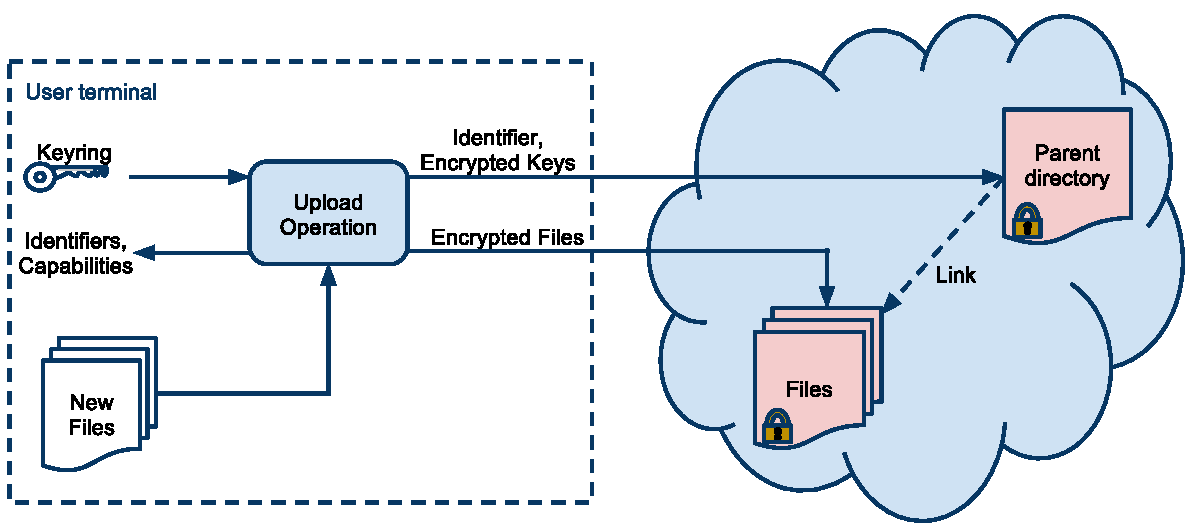
\includegraphics[width=\columnwidth]{ArchitectureUpload.pdf}
    \caption{Scenario: Uploading of files}
    \label{fig:arch:upload}
\end{figure}

\subsection{Download file}

\subsection{Share files}


%**************************************%
\chapter{Cryptographical Solutions}
%**************************************%
This chapter will elaborate on the cryptographical solutions applied to the
architectural scheme in chapter \ref{chap:AS}. We will take a closer look at
how confidentiality, integrity, authentication and access control can be 
integrated into the proposed architecture.\\

A fundamental scheme for key distribution is needed to realize the desired
security features, hence an appropriate solution for key distribution will
also be given.

-Intro - What and why?

{
-Confidentiality: AES-CBC, RSA

-Integrity: SHA-256

-Authentication: RSA PrK signature

-Key hierarchy

-Key distribution
}

%**************************************%
\chapter{Implementation}
%**************************************%

%**************************************%
\chapter{Results}
%**************************************%

%**************************************%
\chapter{Discussion}
%**************************************%

%**************************************%
\chapter{Conclusion and Future Work}
%**************************************%

% BibTeX bibliography lives in external file
\bibliographystyle{plainnat}
\bibliography{references}
% TODO: Can we fix references in order of apperance?

\appendix
\appendixpage
\addappheadtotoc
% Appendix goes here


\end{document}
